\section{Hardware Platform}
The MicroPhase Z7-Lite combines an ARM Cortex-A9 PS and Artix-7-equivalent PL in a single Zynq-7020 SoC. The on-board RTL8201F Ethernet PHY connects to the PS via RGMII, so the MAC and PHY interface are handled entirely within the PS. The PL cannot directly observe raw Ethernet traffic; raw packet bytes must be passed from PS to PL.

\begin{table}[H]
	\centering
	\caption{Z7-Lite PL pin assignments}
	\begin{tabular}{lll}
		\toprule
		\textbf{Signal} & \textbf{Pin} & \textbf{Function} \\
		\midrule
		\texttt{PL\_CLK\_50M} & N18 & 50\,MHz main clock \\
		\texttt{PL\_LED1}     & P15 & \texttt{led\_alert} output \\
		\texttt{GPIO1\_17N}   & U12 & \texttt{led\_active} output \\
		\texttt{PL\_KEY1}     & P16 & Active-low reset \\
		\bottomrule
	\end{tabular}
	\label{tab:pins}
\end{table}

\section{PS-to-PL Packet Forwarding}
The PS ARM receives complete Ethernet frames via the GigE MAC, strips the 4-byte FCS, and writes the frame into a DMA buffer. The AXI-Stream DMA IP transfers the buffer to PL fabric, where \texttt{axis\_rx.vhd} converts AXI-Stream signals (\texttt{tvalid}, \texttt{tready}, \texttt{tdata}, \texttt{tlast}) into the internal byte-stream interface. The entire parser and checker stack is unchanged for hardware use.

\begin{figure}[H]
	\centering
	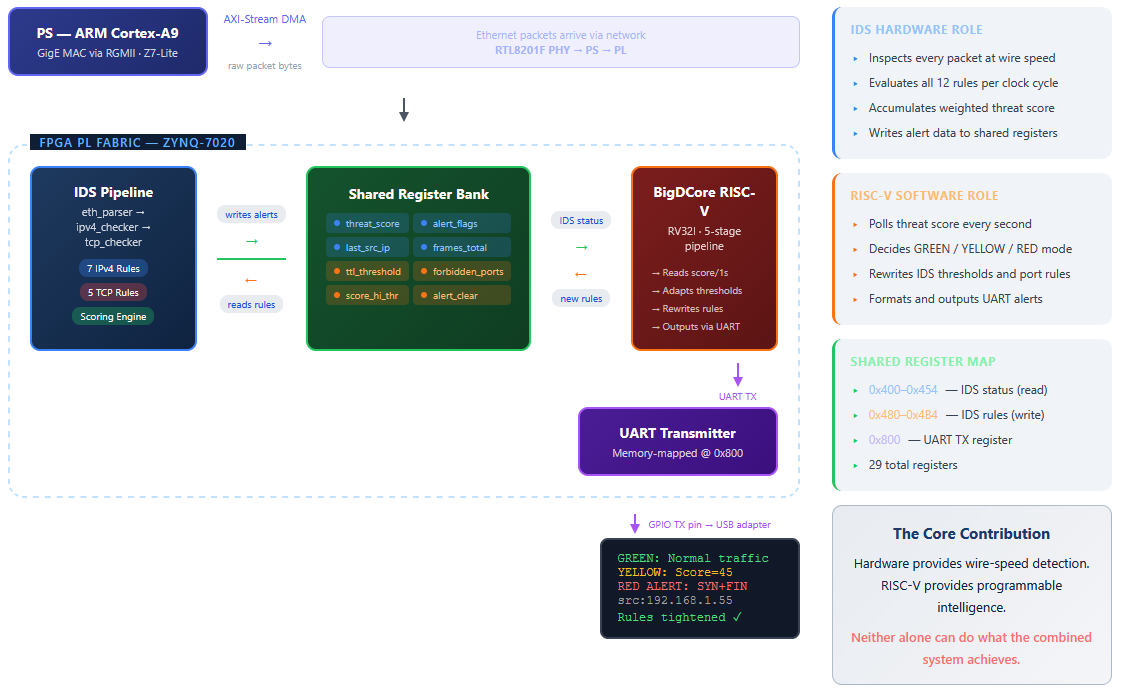
\includegraphics[width=0.95\textwidth]{integration_diagram.png}
	\caption{PS-PL co-design: packet path from RTL8201F through AXI-Stream DMA to the IDS pipeline, with shared register bank connecting IDS to RV32ICore.}
	\label{fig:integration}
\end{figure}

The \texttt{axis\_rx.vhd} wrapper asserts \texttt{tready} permanently and maps: \texttt{tvalid}$\to$\texttt{rx\_valid}, \texttt{tdata[7:0]}$\to$\texttt{rx\_byte}, \texttt{tlast}$\to$\texttt{rx\_eof}, and a one-cycle delayed \texttt{tvalid} rising edge$\to$\texttt{rx\_sof}.

\section{RISC-V Co-Processor Integration}

\subsection{Shared Register Bank}
RV32ICore exposes a standard external memory interface (\texttt{DataAdr}, \texttt{ReadData}, \texttt{WriteData}, \texttt{MemWrite}, \texttt{ByteEn}, \texttt{Mode}), so IDS registers appear to the processor as ordinary memory locations. The shared register bank (\texttt{shared\_regs.vhd}) implements 29 32-bit registers at addresses \texttt{0x400--0x4B4}:

\begin{itemize}
	\item \textbf{Status registers (0x400--0x454)} — written by IDS, read by RISC-V: threat score, 12-bit alert flags bitmask, cumulative alert counts, per-protocol frame counts, frames-per-second statistics, and last-alerted packet fields.
	\item \textbf{Rule registers (0x480--0x4B4)} — written by RISC-V, read by IDS: TTL threshold, fragmentation check enable, scoring thresholds, score decay rate, alert clear command, and eight configurable forbidden port values.
\end{itemize}

\begin{table}[H]
	\centering
	\caption{Shared register map (selected entries)}
	\begin{tabular}{lll}
		\toprule
		\textbf{Address} & \textbf{Register} & \textbf{Direction} \\
		\midrule
		0x400 & \texttt{threat\_score}          & IDS $\rightarrow$ RISC-V \\
		0x404 & \texttt{alert\_flags}           & IDS $\rightarrow$ RISC-V \\
		0x428 & \texttt{fps\_total}             & IDS $\rightarrow$ RISC-V \\
		0x434 & \texttt{last\_alert\_src\_ip}   & IDS $\rightarrow$ RISC-V \\
		0x454 & \texttt{threat\_level}          & IDS $\rightarrow$ RISC-V \\
		0x480 & \texttt{ttl\_threshold}         & RISC-V $\rightarrow$ IDS \\
		0x490 & \texttt{score\_decay\_rate}     & RISC-V $\rightarrow$ IDS \\
		0x494 & \texttt{alert\_clear}           & RISC-V $\rightarrow$ IDS \\
		0x498 & \texttt{forbidden\_port\_0}     & RISC-V $\rightarrow$ IDS \\
		0x800 & \texttt{uart\_tx}               & RISC-V $\rightarrow$ UART \\
		\bottomrule
	\end{tabular}
	\label{tab:regmap}
\end{table}

\subsection{Adaptive Threat Scoring}
The threat score accumulates alert weights each clock cycle and decays by a configurable rate every second. The RISC-V polls the score register at one-second intervals and maps it to three severity levels:

\begin{itemize}
	\item \textbf{GREEN} (score $<$ 30): Normal traffic; default rule thresholds.
	\item \textbf{YELLOW} (30 $\leq$ score $<$ 100): Elevated activity; RISC-V tightens TTL threshold and lowers fragmentation sensitivity.
	\item \textbf{RED} (score $\geq$ 100): Active attack; RISC-V sets maximum TTL threshold and enables all optional checks.
\end{itemize}

\subsection{UART Alert Output}
The RISC-V formats alert data (severity level, triggered rule, source IP) as human-readable strings and transmits them over UART through a memory-mapped transmitter at address \texttt{0x800}.

\section{Packet Capture Module (\texttt{packet\_capture.vhd})}
On each \texttt{frame\_done} pulse, all parsed header fields (Ethernet MACs, EtherType, IPv4 fields, ports, TCP flags, sequence number) are latched into RISC-V-readable registers. A \texttt{capture\_mode} bit selects between logging every frame or only alert-triggering frames.

\section{Future Hardware Integration}
The simulation-verified pipeline is ready for deployment. Remaining steps:
\begin{enumerate}
	\item Create a Vivado block design for xc7z020clg400-1 with Zynq PS configured for GigE MAC with DMA, AXI-Stream DMA IP, and the IDS PL design as a custom IP block.
	\item Write a minimal PS bare-metal C driver in Vitis to forward frames from the GigE MAC to PL via DMA.
	\item Apply XDC constraints from Table~\ref{tab:pins}.
	\item Validate with Scapy-generated test packets over Ethernet.
\end{enumerate}
If hardware integration is not completed before the defense, the simulation results constitute full validation of IDS functionality.